\documentclass[11pt,letterpaper]{article}
\usepackage[margin=0.78in]{geometry}
\usepackage[T1]{fontenc}
\usepackage{amsmath,amssymb}
\usepackage{graphicx}
\usepackage{float}
\usepackage{booktabs}
\usepackage{array}
\usepackage[colorlinks=true,urlcolor=blue,linkcolor=blue]{hyperref}
\setlength{\parskip}{0.38em}
\setlength{\parindent}{0pt}
\emergencystretch=2em
\urlstyle{same}

\newcommand{\repo}{https://github.com/RohMalpani/CS422Assignments/blob/main/assignment4}

\title{CS 422 Assignment 4: Maximum Concurrent Flow and Network Design}
\author{CS 422 project team}
\date{November 2026}

\begin{document}
\maketitle

\section{Submission and code map}
Repository: \href{https://github.com/RohMalpani/CS422Assignments/tree/main/assignment4}{Assignment 4 folder on GitHub}.
\begin{itemize}
\item Part 1 base and loop-rewired constructions:
\href{\repo/part1/topologies.py\#L10-L55}{\texttt{topologies.py}, lines 10--55}.
\item Exact concurrent-flow LP:
\href{\repo/part1/concurrent_flow.py\#L24-L69}{\texttt{concurrent\_flow.py}, lines 24--69}.
\item Upper bound $1/h^*(n,d)$:
\href{\repo/part1/concurrent_flow.py\#L86-L95}{\texttt{concurrent\_flow.py}, lines 86--95}.
\item Part 1 evaluation and figures (one-shot: \texttt{python run.py}):
\href{\repo/part1/run.py\#L51-L170}{\texttt{run.py}, lines 51--170}.
Structural rewiring checks: \href{\repo/part1/test_topologies.py}{\texttt{test\_topologies.py}}.
\item Part 1 true-optimum yardstick for small $n$ (uses the Part 2 MILP):
\href{\repo/part1/optimum_small.py\#L26-L43}{\texttt{optimum\_small.py}, lines 26--43}.
\item Part 2 MILP (Gurobi), whole model:
\href{\repo/part2/topology_milp.py\#L28-L71}{\texttt{topology\_milp.py}, lines 28--71};
variables and objective
\href{\repo/part2/topology_milp.py\#L42-L45}{lines 42--45};
degree, conservation and capacity constraints
\href{\repo/part2/topology_milp.py\#L47-L62}{lines 47--62}.
\item Part 2 hose test matrices:
\href{\repo/part2/run.py\#L45-L89}{\texttt{run.py}, lines 45--89};
evaluation against fixed topologies:
\href{\repo/part2/run.py\#L94-L117}{lines 94--117}
(one-shot: \texttt{python run.py}).
\end{itemize}

\section{Model}
There are $n$ nodes and no other switches. Each node has $d$ outgoing and $d$
incoming directed links of capacity 1. Nodes forward traffic for each other,
and a demand may be split over several paths. Given a traffic matrix $T$, the
concurrent flow $\lambda$ is the largest value such that $\lambda T_{ij}$ can be
routed from $i$ to $j$ for \emph{every} pair at the same time without exceeding
any link capacity.

\section{Part 1: uniform traffic}

\subsection{Upper bound: what any topology can achieve}
Under the uniform matrix $T_{ij}=d/(n-1)$, every node sends $d$ in total, so the
total demand is $nd$, which equals the total link capacity $nd$.

\textbf{Each hop costs capacity.} A unit of flow that travels $h$ hops occupies
one unit of capacity on each of $h$ links. Routing $\lambda T_{ij}$ from $i$ to
$j$ therefore uses at least $\lambda T_{ij}\,\mathrm{dist}(i,j)$ capacity. Summing
over all pairs:
\[
\lambda \frac{d}{n-1}\sum_{i\neq j}\mathrm{dist}(i,j) \;\le\; nd
\quad\Longrightarrow\quad
\lambda \;\le\; \frac{n(n-1)}{\sum_{i\neq j}\mathrm{dist}(i,j)} \;=\; \frac{1}{\bar h(G)},
\]
where $\bar h(G)$ is the average shortest-path hop count. For uniform traffic,
small average hop count is necessary for high $\lambda$, but not sufficient:
routing load must also be balanced. The bound is reached only if (a) all flow
follows shortest paths and (b) every link is fully loaded.

\textbf{No topology has fewer hops than a full $d$-ary tree.} From any node, at
most $d$ nodes are 1 hop away, at most $d^2$ are 2 hops away, and at most $d^h$
are $h$ hops away (the breadth-first argument in the topologies lecture). Filling
these layers greedily, $m_h=\min\!\big(d^h,\,(n-1)-\sum_{k<h}m_k\big)$, gives the
smallest possible average hop count $h^*(n,d)=\frac{1}{n-1}\sum_h h\,m_h$, so
\[
\lambda \;\le\; 1/\bar h(G) \;\le\; 1/h^*(n,d) \qquad\text{for every topology } G.
\]
For example, $n=8,d=4$ gives layers $(4,3)$, $h^*=10/7$, and $\lambda\le 0.7$.
Whether a topology can meet this bound exactly depends on $(n,d)$. It can for
some: our Part~2 MILP reaches it for $n=8,d=4$, and also for $(7,3)$, $(9,4)$,
$(11,2)$ and $(11,5)$ (Table~\ref{tab:p1}). It cannot when $n$ is a ``Moore order''
$1+d+\dots+d^D$ with $d,D\ge2$ (e.g.\ $n=7,d=2$), because perfect directed Moore
graphs do not exist there (Plesn\'ik and Zn\'am, 1974). So in general the goal is a
construction whose hop counts come close to the bound.

\subsection{Construction: loop-rewired generalized de Bruijn graph}
We start with the de Bruijn graph from the topologies lecture (``shift left, then
append one new digit''). Writing it as arithmetic makes it work for any $n$:

\begin{verbatim}
for u in 0 .. n-1:
    for k in 0 .. d-1:
        add link  u -> (d*u + k) mod n
\end{verbatim}

Shifting a base-$d$ label left is multiplying by $d$, and appending digit $k$ is
adding $k$. When $n=d^m$ this is exactly the lecture's de Bruijn graph. Taken mod
$n$, it is the known \emph{generalized de Bruijn digraph} (Reddy, Pradhan and Kuhl,
1980; Imase and Itoh, 1981), which works for any $n$.
Each node has $d$ outgoing links by construction. It also has $d$ incoming links,
because as $u$ ranges over $0..n-1$ and $k$ over $0..d-1$, the values $du+k$ are
exactly the integers $0,\dots,dn-1$. Each residue mod $n$ therefore appears exactly
$d$ times.

\textbf{Where the assumption $d\mid n-1$ is used.} It gives $n\equiv1\pmod d$, so
$\gcd(d,n)=1$, which means $d$ is invertible mod $n$. Then $u\mapsto du \bmod n$ is a
permutation, so each node gets its own block of out-neighbours
$\{du,\dots,du+d-1\}$. Without it the construction degenerates: for $n=8,d=4$
($\gcd=4$), every even node has the same four out-neighbours $\{0,1,2,3\}$, every
odd node has $\{4,\dots,7\}$, and 4 of the 32 ports are self-loops (we see the cost
in Part~2). The assumption also rules out $n=d^m$, which is why the mod-$n$
generalization is needed in the first place.

\textbf{Rewiring wasted ports.} List the base graph's self-loop nodes in
increasing order $s_0,\ldots,s_{q-1}$; remove each $s_i\to s_i$ and add
$s_i\to s_{(i+1)\bmod q}$. In our $d\mid n-1$ setting, these are distinct single
loops and $q\ge2$. Each affected node loses one incoming and one outgoing link,
then gains one of each from the directed cycle. Thus every node still has
exactly $d$ incoming and $d$ outgoing unit-capacity links, with no self-loops.
The new edge may be parallel to an existing edge; the capacity matrix records
both. This is a deterministic improvement heuristic, \emph{not} a proof of the
best topology for arbitrary $(n,d)$. Figure~\ref{fig:db} shows both versions at
$n=9,d=2$.

\begin{figure}[h]
\centering
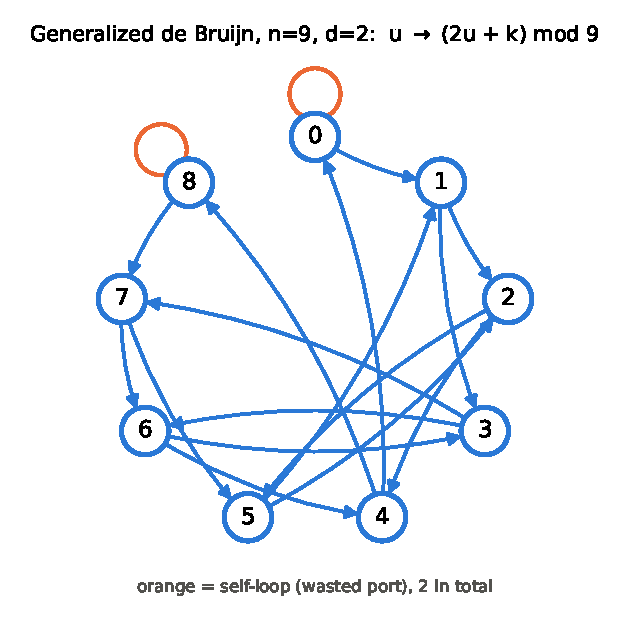
\includegraphics[width=0.43\linewidth]{figures/part1_debruijn_n9_d2.pdf}\hfill
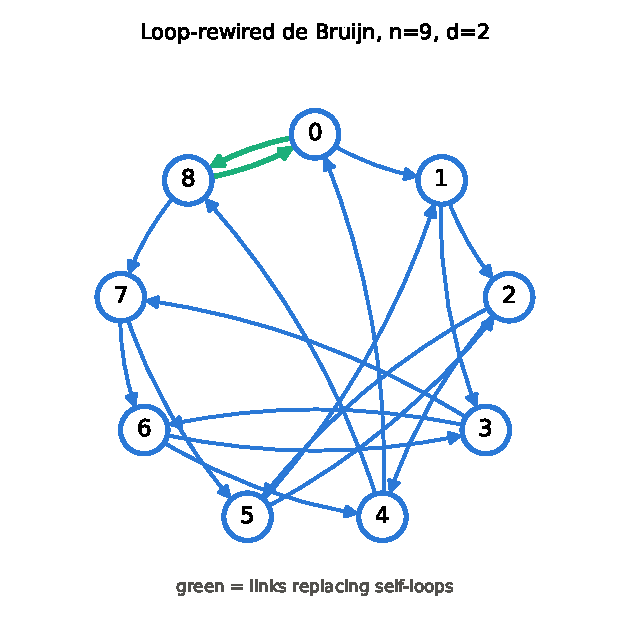
\includegraphics[width=0.43\linewidth]{figures/part1_rewired_n9_d2.pdf}
\caption{Base (left) and loop-rewired (right) de Bruijn graphs for $n=9,d=2$.
Orange rings are wasted self-loop ports; green edges replace them.}
\label{fig:db}
\end{figure}

\subsection{Why start from de Bruijn: short paths}
\textbf{In the base graph, every node reaches every other in at most
$\lceil\log_d n\rceil$ hops.}
After $m$ hops from $u$ with digits $k_1,\dots,k_m$ we are at
\[
d^m u + (k_1 d^{m-1} + k_2 d^{m-2} + \dots + k_m) \pmod n .
\]
The bracketed term can be any integer in $0,\dots,d^m-1$, the base-$d$ numbers
with $m$ digits. Once $d^m\ge n$, these cover every residue mod $n$, so every
target is reachable. The breadth-first lower bound says no topology can reach
all $n$ nodes in fewer than about $\log_d n$ hops, so de Bruijn's diameter is
within one hop of the smallest possible: it grows logarithmically, as the best
possible does. For
comparison, the obvious ``ring with chords'' (simple circulant
$u\to u+1,\dots,u+d$) reaches only $d$ new nodes per hop, so its average hop
count grows linearly in $n$.
Removing self-loops cannot remove a shortest path between distinct nodes, and
the rewiring only adds usable links. Therefore the rewired graph retains the
same $\lceil\log_d n\rceil$ diameter guarantee.

\subsection{Why this is a strong general construction}
The topology is explicit for every admissible $(n,d)$: it preserves exactly $d$
incoming and $d$ outgoing ports at every node, eliminates unusable self-loops,
and retains the logarithmic diameter proved above. The Moore-style breadth-first
bound shows that no degree-$d$ topology can have substantially smaller diameter
as $n$ grows. Short paths matter because every additional hop consumes another
unit of link capacity for the same delivered traffic.

The rewiring also \emph{cannot reduce} maximum concurrent flow relative to the
base graph. A feasible flow never needs a self-loop: deleting self-loop flow
does not alter conservation or delivery. All non-loop capacities of the base
graph remain and some increase, so every feasible base routing is still
feasible after rewiring. Thus $\lambda_{\mathrm{rewired}}\ge
\lambda_{\mathrm{base}}$ for every traffic matrix, not just the tested uniform
ones. This is a reason to use the rewired construction, rather than a claim
that it always attains the global optimum.

\textbf{What ``close to optimal'' means here.} Let $C$ be the exact LP value of
our rewired graph, $O$ the best value over all feasible topologies, and
$U=1/h^*(n,d)$ the universal hop-capacity upper bound. Since
$C\le O\le U$, we have
\[
\frac{C}{O}\ge\frac{C}{U}.
\]
The measured ratio $C/U$ is therefore a rigorous \emph{lower bound on the
fraction of the unknown optimum achieved} for each tested $(n,d)$; it is not
merely a comparison with another heuristic. For small cases, the Part~2 MILP
also supplies $O$ directly (or a range) for a sharper check. Neither the
short-path property nor this finite set of measurements proves the rewired
graph is exactly best for every $(n,d)$: uneven link load can still force
detours. A globally optimal construction would require a matching lower-bound
proof for all parameters.

\subsection{Evaluation}
For 15 admissible pairs $(n,d)$ we computed $C$ with the Gurobi concurrent-flow
LP (one commodity per source, arc-flow conservation and capacity constraints).
The black marks in Figure~\ref{fig:lambda} are $U$, an upper bound on \emph{any}
topology; green dots are the achieved $C$. Table~\ref{tab:p1} reports the
certified fraction $C/U$. The CSV also retains the original de Bruijn and
circulant values for reproducibility, but the central question is how close
our construction is to the global optimum.

\begin{figure}[h]
\centering
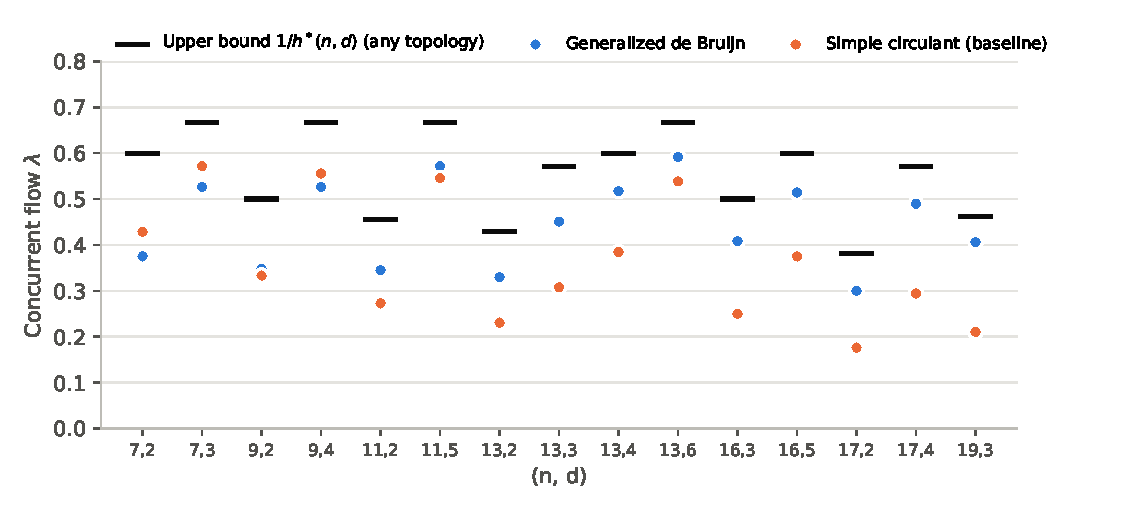
\includegraphics[width=0.92\linewidth]{figures/part1_lambda_vs_bound.pdf}
\caption{Achieved concurrent flow $C$ for the loop-rewired construction versus
the universal upper bound $U$ on any topology. The vertical gap is an upper
bound on how much optimality remains possible.}
\label{fig:lambda}
\end{figure}

\begin{table}[H]
\centering\footnotesize\setlength{\tabcolsep}{5pt}
\begin{tabular}{rrcccc}
\toprule
$n$ & $d$ & upper bound $U$ & achieved $C$ & certified $C/U$ & MILP bound on optimum $O$ \\
\midrule
 7 & 2 & 0.600 & 0.429 & 71\% & 0.545 \\
 7 & 3 & 0.667 & 0.632 & 95\% & 0.667 \\
 9 & 2 & 0.500 & 0.387 & 77\% & 0.488--0.500 \\
 9 & 4 & 0.667 & 0.606 & 91\% & 0.667 \\
11 & 2 & 0.455 & 0.370 & 81\% & 0.455 \\
11 & 5 & 0.667 & 0.625 & 94\% & 0.667 \\
13 & 2 & 0.429 & 0.349 & 81\% & -- \\
13 & 3 & 0.571 & 0.505 & 88\% & -- \\
13 & 4 & 0.600 & 0.567 & 94\% & -- \\
13 & 6 & 0.667 & 0.629 & 94\% & -- \\
16 & 3 & 0.500 & 0.451 & 90\% & -- \\
16 & 5 & 0.600 & 0.552 & 92\% & -- \\
17 & 2 & 0.381 & 0.318 & 83\% & -- \\
17 & 4 & 0.571 & 0.531 & 93\% & -- \\
19 & 3 & 0.462 & 0.439 & 95\% & -- \\
\bottomrule
\end{tabular}
\caption{Part 1 evidence (\texttt{part1/results/part1.csv}). Since $O\le U$,
the $C/U$ column certifies at least that fraction of the best possible $O$.
The small-instance MILP (\texttt{part1/results/part1\_optimum.csv}) gives
exact $O$ where shown, except $(9,2)$ where its time limit leaves a range.
Percentages use unrounded LP and bound values.}
\label{tab:p1}
\end{table}

\textbf{How close is it?}
\begin{itemize}
\item In every tested case, the construction achieves at least 71\% of the
unknown global optimum by the $C/U$ certificate; in 9 of 15 cases the
certificate is at least 90\%. The strongest certified case is $(19,3)$:
$C=0.439$ versus $U=0.462$, so even the best topology can improve concurrent
flow by no more than about 5\% of its own value.
\item The small-instance MILP sharpens that comparison. For $(7,3)$,
$C/O=0.632/0.667\approx95\%$; for $(9,4)$ it is about 91\%. The weakest
proven case is $(7,2)$, where $0.429/0.545\approx79\%$. At $(9,2)$, the
time-limited MILP places $O$ between 0.488 and 0.500, so $C/O$ is between
about 77\% and 79\%.
\item No measured case reaches a proved global optimum. The remaining gap
is real in small cases, not just looseness of the Moore bound. The construction
is therefore a reproducible near-optimal candidate with a quantified gap,
not an exact solution to the general topology-optimization problem.
\end{itemize}

\section{Part 2: arbitrary hose traffic ($n=8$, $d=4$)}
We present a \textbf{mixed-integer linear program}. Given one traffic matrix
$T\in\mathcal{T}_{\text{hose}}$, it chooses the topology and the routing
together. The topology \emph{adapts} to $T$ because the program is solved again for
each new $T$, as a reconfigurable (e.g.\ optical circuit-switched) network would
pick a new set of circuits.

\subsection{Formulation}
Let $V=\{0,\dots,7\}$, $A=\{(u,v): u,v\in V,\ u\neq v\}$ and $d=4$.

\textbf{Decision variables.}
\begin{itemize}
\item $x_{uv}\in\{0,1,\dots,d\}$ for $(u,v)\in A$: number of unit-capacity links
from $u$ to $v$, i.e.\ \emph{the topology}. It is integer because a link cannot be
half-built. Values above 1 are parallel links.
\item $f^s_{uv}\ge0$ for $s\in V$, $(u,v)\in A$: traffic that originated at source
$s$ and crosses link $u\to v$, i.e.\ \emph{the routing}.
\item $\lambda\ge0$: the fraction of every demand that is delivered.
\end{itemize}

\textbf{Objective.} $\displaystyle\max\ \lambda$.

\textbf{Constraints.}
\begin{align}
\textstyle\sum_{v\neq u} x_{uv} &= d \quad \forall u\in V,
&\textstyle\sum_{u\neq v} x_{uv} &= d \quad \forall v\in V
&& \text{(degree)}\\
\textstyle\sum_{w\neq v} f^s_{vw}-\sum_{u\neq v} f^s_{uv} &=
\begin{cases}\lambda\sum_t T_{st} & v=s\\ -\lambda T_{sv} & v\neq s\end{cases}
&& \forall s,v\in V
&& && \text{(conservation)}\\
\textstyle\sum_{s\in V} f^s_{uv} &\le x_{uv} && \forall (u,v)\in A
&& && \text{(capacity)}
\end{align}

\subsection{Intuition}
\begin{itemize}
\item With $x$ \emph{fixed}, constraints (2)--(3) are exactly the concurrent-flow
LP we use in Part~1 to evaluate a topology. Source $s$ emits $\lambda$ times its
total demand, each destination $v$ absorbs $\lambda T_{sv}$, and every other node
forwards what it receives (net zero). Flow may be split and may take any number
of hops.
\item Making $x$ a \emph{variable}, limited only by the port budget (1), lets the
solver search over every topology with $d$ outgoing and $d$ incoming links at
the same time as the routing. The optimum is therefore the largest $\lambda$
achievable by \emph{any} such topology for this $T$. That is exactly ``the topology
that maximizes concurrent flow for the given traffic matrix''.
\item The model is linear: $\lambda T_{st}$ is a variable times a constant, and
capacity compares flows with $x$. Only $x$ is integer, so it is a MILP. Gurobi
proves optimality up to its default tolerance (0.01\% MIP gap), and our script
asserts this for every solve instead of accepting a time-limited answer.
\item Self-loops are excluded because they cannot carry traffic. Parallel links
are allowed and necessary: for $T=4\times$ a permutation, the optimum puts all 4
links on each node's single destination and reaches $\lambda=1$.
\item One commodity per \emph{source} (8 commodities) instead of per pair (56)
gives the same $\lambda$, because a single-source flow decomposes into paths to
each destination. This keeps the model at 56 integer and 449 continuous variables.
\item \textbf{Upper bound.} We test matrices whose row and column sums are
exactly 4, the fully loaded case. Total demand is then $32$, which equals total
capacity $8\cdot4$, so $\lambda\le1$, with equality only if every demand travels
one hop. The hose set also allows smaller sums. The model handles those unchanged,
and $\lambda$ can then exceed 1. The only exception is $T=0$, where every $\lambda$
is feasible, so the code rejects it.
\end{itemize}

\subsection{Evaluation}
We solved the MILP for 15 hose matrices, each with every row and column summing
to 4 and a zero diagonal:
\begin{itemize}
\item a $4\times$ permutation;
\item two permutations with weight 2;
\item three permutations with real weights $(0.5,0.3,0.2)\times4$, chosen so that no two send to the same destination from the same source;
\item a skewed matrix (3 to one partner plus 1 spread uniformly);
\item the uniform matrix;
\item 10 random dense matrices (uniform random entries scaled by Sinkhorn
iteration to row/column sums of 4, seed 422).
\end{itemize}
Every MILP solution was re-scored by the independent Part~1 LP, and the two
$\lambda$ values agree. As baselines that do \emph{not} adapt, we fixed two topologies and
evaluated them on every matrix with the same LP: (i) the MILP-optimal topology
for the uniform matrix, chosen once, and (ii) the \emph{original} (not rewired)
Part~1 de Bruijn graph for
$n=8,d=4$ (Figure~\ref{fig:p2}).

\begin{figure}[h]
\centering
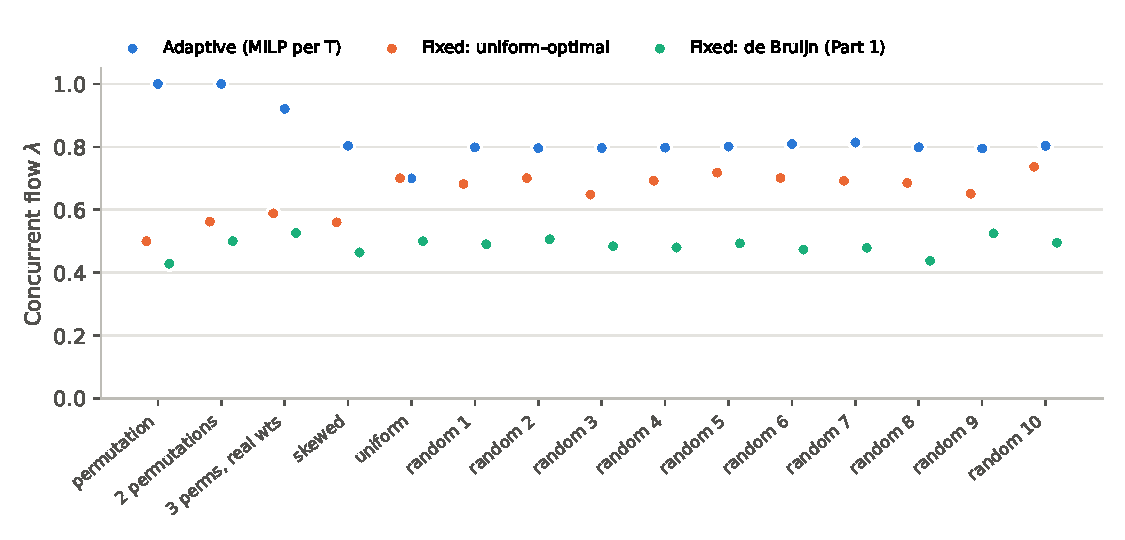
\includegraphics[width=0.92\linewidth]{figures/part2_lambda.pdf}
\caption{Concurrent flow per hose matrix: topology re-optimized for each $T$ vs.\
two fixed topologies. Every MILP solve was proven optimal (gap 0 within
Gurobi's 0.01\% tolerance, checked in code).}
\label{fig:p2}
\end{figure}

\begin{table}[h]
\centering\small
\begin{tabular}{lccc}
\toprule
Matrix & adaptive (MILP) & fixed: uniform-optimal & fixed: de Bruijn \\
\midrule
$4\times$ permutation & 1.000 & 0.542 & 0.417 \\
2 permutations & 1.000 & 0.625 & 0.450 \\
3 perms, real weights & 0.938 & 0.676 & 0.476 \\
skewed & 0.803 & 0.587 & 0.461 \\
uniform & 0.700 & 0.700 & 0.500 \\
random (10, mean / range) & 0.799 / 0.775--0.812 & 0.678 / 0.610--0.701 & 0.509 / 0.487--0.541 \\
\bottomrule
\end{tabular}
\caption{Part 2 results (\texttt{part2/results/part2.csv}).}
\label{tab:p2}
\end{table}

\textbf{Findings.}
\begin{itemize}
\item \textbf{Integer-structured traffic is served perfectly.} If $T$ is an integer
combination of permutations, the MILP builds exactly those direct links (with
parallel links where needed) and reaches $\lambda=1$, the upper bound.
\item \textbf{Fractional traffic needs some relaying.} For the three-permutation
matrix (Figure~\ref{fig:adapt}), each demand of 2.0 gets 2 links, but demands of
1.2 and 0.8 can only get 1 link each, since links are whole units and each node has
only 4. Part of every 1.2 demand must then travel two hops, using spare capacity on
other links (such as the 0.8 links). Two-hop flow costs double capacity, so
$\lambda=0.938<1$.
\item \textbf{Uniform is the hardest of the matrices we tested.} This is an
observation from our 15 samples, not a proof over the whole hose set. The MILP
reaches $\lambda=0.7$, exactly Part~1's bound $1/h^*(8,4)$, so the bound is tight
for $n=8,d=4$ (the optimal topology has average hop count exactly $10/7$). Random
dense matrices land in between ($\approx0.80$).
\item \textbf{Adapting pays off.} A fixed topology can be good for one kind of
traffic but not for all. The uniform-optimal topology matches the MILP on uniform
traffic but delivers only about half of a permutation (0.542). On random
matrices, adapting gives 18\% more $\lambda$ on average. De Bruijn is worst here
because $n=8,d=4$ violates Part~1's assumption $d\mid n-1$: $\gcd(4,8)=4$, so the
construction degenerates (Section~3.2). Every even node has the same four
out-neighbours, and 4 of the 32 ports are self-loops.
\end{itemize}

\begin{figure}[h]
\centering
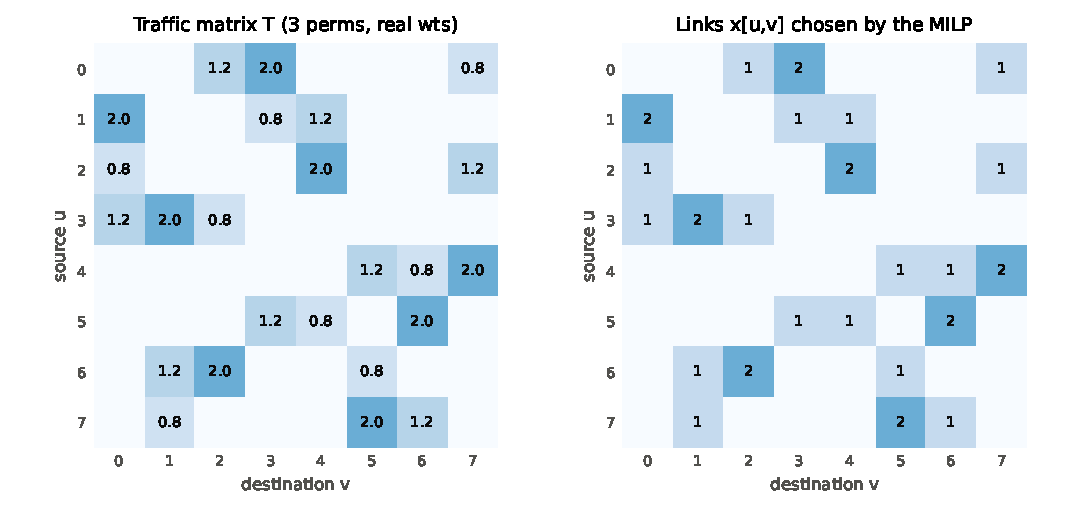
\includegraphics[width=0.85\linewidth]{figures/part2_adapt_example.pdf}
\caption{The topology follows the demand: three-permutation matrix (left) and
the link counts the MILP chooses for it (right), $\lambda=0.938$.}
\label{fig:adapt}
\end{figure}

\section{AI use}
Claude (Claude Code) was used interactively during the initial implementation
for conceptual guidance (concurrent flow, the hop-count bound, mapping lecture
slides to the problem), proposing and comparing candidate topologies, and
drafting the Gurobi LP/MILP code, evaluation scripts, figures, and report text.
Codex assisted with the later loop-rewiring implementation, structural tests,
LP reruns, figure regeneration, and this report update. The code was validated
against hand-computed cases (complete graph, directed ring, permutation,
uniform bound) and the measured data in the repository. Decisions and rationale
are logged in \texttt{DECISIONS.md}, and AI use in \texttt{AI\_USAGE.md}.

\end{document}
